%% ============================================================
%%  CMP4509 Term Project Report
%%  Understanding Deep Learning Requires Rethinking Generalization:
%%  A Reproduction Study
%% ============================================================
\documentclass[12pt,a4paper]{article}

%% ---------- Packages ----------
\usepackage[margin=2.5cm]{geometry}
\usepackage[T1]{fontenc}
\usepackage[utf8]{inputenc}
\usepackage{lmodern}
\usepackage{amsmath}
\usepackage{amssymb}
\usepackage{amsthm}
\usepackage{graphicx}
\usepackage{booktabs}
\usepackage[colorlinks=true,linkcolor=blue!70!black,citecolor=green!50!black,urlcolor=blue]{hyperref}
\usepackage{xcolor}
\usepackage[most]{tcolorbox}
\usepackage[backend=bibtex,style=numeric,sorting=nyt]{biblatex}
\usepackage{cleveref}
\usepackage{subcaption}
\usepackage{siunitx}

\addbibresource{references.bib}

%% ---------- Guide-box toggle ----------
\newif\ifshowguides
\showguidestrue   % Set to \showguidesfalse to hide all guide boxes before submission

\newcommand{\guide}[1]{%
  \ifshowguides
    \begin{tcolorbox}[colframe=blue!60,colback=blue!5,
                      title={\small\textbf{Instructor Guide}},
                      fonttitle=\small\bfseries]
      {\small\textit{Guide: }#1}
    \end{tcolorbox}
  \fi
}

%% ---------- Theorem environments ----------
\newtheorem{theorem}{Theorem}[section]
\newtheorem{lemma}[theorem]{Lemma}
\newtheorem{corollary}[theorem]{Corollary}
\theoremstyle{definition}
\newtheorem{definition}[theorem]{Definition}
\theoremstyle{remark}
\newtheorem{remark}[theorem]{Remark}

%% ---------- Title metadata ----------
\title{%
  \textbf{Understanding Deep Learning Requires Rethinking Generalization:}\\
  \large A Reproduction Study\\[0.5em]
  {\normalsize CMP4509 Introduction to Deep Learning --- Term Project Report}
}
\author{
  Emirhan Kılıç\\
  {\small Department of Computer Engineering}\\
  {\small \texttt{emirhan.kilic1@bahcesehir.edu.tr}}
  \and
  Yakup Nail Ceylan\\
  {\small Department of Computer Engineering}\\
  {\small \texttt{yakupnail.ceylan@bahcesehir.edu.tr}}
  \and
  Ahmet Erbey\\
  {\small Department of Computer Engineering}\\
  {\small \texttt{ahmet.erbey@bahcesehir.edu.tr}}
}
\date{\today}

%% ============================================================
\begin{document}
\maketitle

%% ---------- Abstract ----------
\begin{abstract}
Zhang et al.~\cite{zhang2017understanding} demonstrated that standard deep
neural networks possess sufficient capacity to memorize entire datasets with
randomized labels, achieving near-zero training error while maintaining
meaningful generalization on clean data. This challenges conventional wisdom
that explicit regularization is the primary driver of generalization. In this
reproduction study for CMP4509, we re-implement the core randomization and
corruption experiments from Section~2 of the paper using CIFAR-10~\cite{krizhevsky2009learning}
with a $5{,}158{,}730$-parameter convolutional network (SmallCNN) and an MLP-512
trained with standard mini-batch SGD (momentum $= 0.9$, learning rate $= 0.01$,
without explicit regularizers or data augmentation) for $40$ epochs across three
random seeds ($42, 123, 456$). We sweep label corruption rates
$\alpha \in \{0.0, 0.2, 0.4, 0.6, 0.8, 1.0\}$ and test four input-corruption
modes (true pixels, shuffled pixels, random pixels, Gaussian noise). Our empirical
results confirm the paper's central findings: on clean labels ($\alpha = 0.0$),
SmallCNN achieves $100.00 \pm 0.00\%$ training accuracy and $83.97 \pm 0.17\%$
test accuracy (converging in $11.0 \pm 0.0$ epochs). As label corruption increases,
test error degrades monotonically ($16.03\%$ error at $\alpha=0.0 \to 30.77\%$ at
$\alpha=0.2 \to 50.01\%$ at $\alpha=0.4 \to 69.44\%$ at $\alpha=0.6 \to 78.93\%$
at $\alpha=0.8 \to 90.00\%$ at $\alpha=1.0$), while the network still fits up to
$73.91 \pm 0.98\%$ of the training data even at $80\%$ label corruption and exhibits
substantial optimization slowdown ($2.21\times$ slower to reach $95\%$ training
accuracy at $\alpha=0.2$, and $2.94\times$ at $\alpha=0.4$). Furthermore, we provide
a complete, constructive derivation and numerical verification of Theorem~1
($p = 2n + d$), showing that finite-sample expressivity is achievable with far
fewer parameters than modern deep architectures possess.
\end{abstract}

\tableofcontents
\clearpage

%% ============================================================
\section{Introduction}
\label{sec:intro}
%% ============================================================

\guide{%
  The introduction should (1)~motivate the research question, (2)~state the
  exact testable claim of the reproduced paper, (3)~explain \emph{why} the
  claim is surprising, (4)~outline the structure of the remainder of the
  report. Cite the original paper and any directly relevant background.
  Aim for 300--500 words.
}

A fundamental question in deep learning is: \emph{why do over-parameterized
neural networks generalize at all?} Classical statistical learning theory
bounds generalization error via complexity measures such as VC dimension or
Rademacher complexity; networks with millions of parameters and zero
training error should, by those bounds, generalize poorly. Yet in practice
they do not.

Zhang et al.~\cite{zhang2017understanding} provided a striking empirical
answer. Their central, \textbf{testable claim} (presented in Section~2 and
Figure~1 of the original paper) is:

\begin{quote}
  Standard deep networks can fit training data with \emph{randomized labels}
  and unstructured inputs to near-zero training error, yet they generalize well
  on real data without changing the architecture, optimizer, or hyperparameters.
  As the label corruption rate $\alpha$ increases from $0$ to $1$, test error
  grows smoothly while optimization convergence slows down by a constant factor.
\end{quote}

This finding shows that the same architecture and optimizer that achieves
strong test accuracy on true CIFAR-10 labels can also memorize corrupted
labels when no semantic signal exists. The network's parameter count therefore
cannot be the \emph{reason} it generalizes --- another mechanism, related to the
interaction between the data distribution, the architecture, and the implicit
regularization of stochastic gradient descent, must be responsible.

The implications are twofold. First, explicit regularizers (dropout, weight
decay, data augmentation) improve test performance as tuning knobs but are
\emph{neither necessary nor sufficient} to control generalization error.
Second, understanding generalization requires theoretical tools beyond
label-independent uniform convergence bounds~\cite{goodfellow2016deep}.

In this report we reproduce the core randomization experiments on
CIFAR-10~\cite{krizhevsky2009learning} with a compute-budget-friendly
SmallCNN and MLP-512, covering:
\begin{itemize}
  \item \textbf{E1}: Clean baseline ($\alpha = 0.0$), fully randomized labels
        ($\alpha = 1.0$), and input corruption modes (shuffled pixels, random
        pixels, Gaussian noise).
  \item \textbf{E2}: Label corruption sweep across
        $\alpha \in \{0.0, 0.2, 0.4, 0.6, 0.8, 1.0\}$.
\end{itemize}
We additionally provide a formal proof of the finite-sample expressivity
theorem (\Cref{sec:background}), a full description of the experimental
setup (\Cref{sec:setup}), results and discussion (\Cref{sec:results}), and
conclusions (\Cref{sec:conclusion}).

%% ============================================================
\section{Background and Method}
\label{sec:background}
%% ============================================================

%% ----------------------------------------------------------
\subsection{Problem Setup}
\label{sec:problem}
%% ----------------------------------------------------------

\guide{%
  Define the learning problem formally. Introduce the dataset, the
  corruption procedure, and the notation you will use throughout.
  Include any equations that make the setup precise.
}

\paragraph{Dataset.}
CIFAR-10~\cite{krizhevsky2009learning} consists of $60{,}000$ color images
of size $32 \times 32 \times 3$ distributed uniformly over $C = 10$ classes
($50{,}000$ training, $10{,}000$ test). Each image is represented as a vector
$\mathbf{x} \in [0,1]^d$ where $d = 32 \times 32 \times 3 = 3{,}072$.

\paragraph{Label corruption.}
Let $\mathcal{D} = \{(\mathbf{x}_i, y_i)\}_{i=1}^{n}$ be the training set
with $y_i \in \{0,\ldots,C{-}1\}$. Given a corruption rate
$\alpha \in [0,1]$, we construct a corrupted label set by drawing, for a
random subset of $\lfloor \alpha n \rfloor$ indices, a replacement label
uniformly from $\{0,\ldots,C{-}1\}$:
\begin{equation}
  \tilde{y}_i =
  \begin{cases}
    \mathrm{Uniform}(\{0,\ldots,C{-}1\}) & \text{if } i \in \mathcal{S},\\
    y_i & \text{otherwise,}
  \end{cases}
  \label{eq:corruption}
\end{equation}
where $|\mathcal{S}| = \lfloor \alpha n \rfloor$ and $\mathcal{S}$ is drawn
uniformly at random (without replacement) before training. At $\alpha = 0$
no labels are corrupted; at $\alpha = 1$ all labels are independently
randomized.

\paragraph{Input corruption.}
We additionally consider four input-corruption modes:
\begin{enumerate}
  \item \textbf{True}: original CIFAR-10 pixels --- no input corruption.
  \item \textbf{Shuffled pixels}: a single fixed permutation $\pi$ of the
        $d$ pixel positions is drawn once and applied to every image.
  \item \textbf{Random pixels}: each pixel of each image is resampled
        independently from $\mathrm{Uniform}([0,1])$.
  \item \textbf{Gaussian noise}: each pixel is drawn from
        $\mathcal{N}(0.5,\, 0.5^2)$ and clamped to $[0,1]$.
\end{enumerate}

%% ----------------------------------------------------------
\subsection{Architecture}
\label{sec:arch}
%% ----------------------------------------------------------

\paragraph{SmallCNN.}
Inspired by the Inception-style CNN used in the original paper but scaled
down for our compute budget, SmallCNN consists of four convolutional blocks
with Batch Normalization (BN) followed by two fully-connected layers:
\begin{align}
  &\text{Conv}(3 \to 64,\, 3{\times}3,\, \mathrm{pad}{=}1) \to \mathrm{BN} \to \mathrm{ReLU} \notag\\
  &\text{Conv}(64 \to 128,\, 3{\times}3,\, \mathrm{pad}{=}1) \to \mathrm{BN} \to \mathrm{ReLU} \to \mathrm{MaxPool}(2) \notag\\
  &\text{Conv}(128 \to 256,\, 3{\times}3,\, \mathrm{pad}{=}1) \to \mathrm{BN} \to \mathrm{ReLU} \notag\\
  &\text{Conv}(256 \to 256,\, 3{\times}3,\, \mathrm{pad}{=}1) \to \mathrm{BN} \to \mathrm{ReLU} \to \mathrm{MaxPool}(2) \notag\\
  &\mathrm{Flatten} \to \mathrm{Linear}(256 \cdot 8 \cdot 8,\, 256) \to \mathrm{ReLU} \to \mathrm{Linear}(256,\, 10).
  \label{eq:cnn}
\end{align}
Including convolutional kernels, bias vectors, Batch Normalization affine
parameters, and linear layers, the exact trainable parameter count is:
\begin{equation}
  p_{\mathrm{CNN}} = 5{,}158{,}730 \approx 5.16 \times 10^6.
  \label{eq:cnn_params}
\end{equation}

\paragraph{MLP-512.}
A single-hidden-layer multilayer perceptron with $512$ units:
\begin{equation}
  f_{\mathrm{MLP}}(\mathbf{x}) =
    \mathbf{W}_2\, \mathrm{ReLU}(\mathbf{W}_1 \mathbf{x} + \mathbf{b}_1) + \mathbf{b}_2,
  \label{eq:mlp}
\end{equation}
where $\mathbf{W}_1 \in \mathbb{R}^{512 \times 3072}$,
$\mathbf{b}_1 \in \mathbb{R}^{512}$,
$\mathbf{W}_2 \in \mathbb{R}^{10 \times 512}$,
$\mathbf{b}_2 \in \mathbb{R}^{10}$, giving
$p_{\mathrm{MLP}} = 512{\cdot}3072 + 512 + 10{\cdot}512 + 10 = 1{,}578{,}506$
parameters.

%% ----------------------------------------------------------
\subsection{Theorem 1: Finite-Sample Expressivity of 2-Layer ReLU Networks}
\label{sec:theorem}
%% ----------------------------------------------------------

\guide{%
  This subsection provides the formal theorem and proof sketch from
  Zhang et al.\ (2017). Ensure every symbol is defined before it is used.
  Walk through each step of the construction clearly. You may use the
  \texttt{proof} environment from \texttt{amsthm}.
}

We now state and prove the key theoretical result that underpins the
experimental observations.

\begin{theorem}[Universal finite-sample representation]
\label{thm:representation}
  Let $n, d \in \mathbb{N}$ with $n \geq 1$. There exists a 2-layer ReLU
  network with
  \begin{equation}
    p = 2n + d
    \label{eq:param_count}
  \end{equation}
  parameters that can represent \emph{any} function
  $f : \{\mathbf{x}_1, \ldots, \mathbf{x}_n\} \to \mathbb{R}$
  on $n$ distinct points $\mathbf{x}_1, \ldots, \mathbf{x}_n \in \mathbb{R}^d$.
\end{theorem}

\noindent
\textbf{Symbol glossary:}
\begin{itemize}
  \item $n \in \mathbb{N}$ --- number of training samples ($n = 50{,}000$ for CIFAR-10).
  \item $d \in \mathbb{N}$ --- input dimension ($d = 3{,}072$ for CIFAR-10).
  \item $p \in \mathbb{N}$ --- total parameter count of the constructed network.
  \item $\mathbf{x}_i \in \mathbb{R}^d$ --- the $i$-th training point.
  \item $y_i \in \mathbb{R}$ --- the target label for $\mathbf{x}_i$.
  \item $\mathbf{a} \in \mathbb{R}^d$ --- a shared projection direction vector.
  \item $z_i = \mathbf{a}^\top \mathbf{x}_i \in \mathbb{R}$ --- the projected scalar for point $i$.
  \item $b_j \in \mathbb{R}$ --- bias threshold of hidden unit $j$ ($j = 1,\ldots,n$).
  \item $w_j \in \mathbb{R}$ --- output weight of hidden unit $j$.
  \item $\mathbf{A} \in \mathbb{R}^{n \times n}$ --- hidden activation matrix used in the construction.
\end{itemize}

\begin{proof}[Proof sketch]
\textbf{Step 1: Choose a generic projection direction.}
Draw $\mathbf{a} \in \mathbb{R}^d$ uniformly at random from the unit sphere.
Define $z_i = \mathbf{a}^\top \mathbf{x}_i$ for $i = 1,\ldots,n$.
Because the $\mathbf{x}_i$ are distinct and $\mathbf{a}$ is drawn from a continuous
distribution, the values $z_1,\ldots,z_n$ are distinct with probability~$1$.
Relabel the indices so that $z_1 < z_2 < \cdots < z_n$.

\textbf{Step 2: Place biases to separate the projections.}
Choose biases $b_1 < b_2 < \cdots < b_n$ such that
\begin{equation}
  b_j < z_j < b_{j+1} \quad \text{for all } j = 1,\ldots,n-1,
  \quad b_1 < z_1.
  \label{eq:bias_interleave}
\end{equation}
Such a choice is always possible since the $z_i$ are strictly ordered.

\textbf{Step 3: Construct the activation matrix.}
Define $\mathbf{A} \in \mathbb{R}^{n \times n}$ by
\begin{equation}
  A_{ij} = \max(z_i - b_j,\; 0), \qquad i,j = 1,\ldots,n.
  \label{eq:activation_matrix}
\end{equation}
By the interleaving property~\eqref{eq:bias_interleave}:
\begin{itemize}
  \item $A_{ij} = 0$ whenever $j > i$ (since $z_i < b_j$ when $j > i$),
        making $\mathbf{A}$ \emph{lower triangular}.
  \item $A_{ii} = z_i - b_i > 0$ for all $i$, so all diagonal entries are strictly
        positive.
\end{itemize}
Since $\det(\mathbf{A}) = \prod_{i=1}^n A_{ii} > 0$, $\mathbf{A}$ is invertible.

\textbf{Step 4: Solve for output weights.}
Because $\mathbf{A}$ is invertible, the linear system
\begin{equation}
  \mathbf{A}\,\mathbf{w} = \mathbf{y}, \qquad
  \mathbf{w} = (w_1,\ldots,w_n)^\top \in \mathbb{R}^n,\quad
  \mathbf{y} = (y_1,\ldots,y_n)^\top \in \mathbb{R}^n
  \label{eq:linear_system}
\end{equation}
has a unique solution $\mathbf{w} = \mathbf{A}^{-1}\mathbf{y}$.

\textbf{Step 5: Verify parameter count.}
The constructed network is
\begin{equation}
  f(\mathbf{x}) = \sum_{j=1}^{n} w_j\, \max\!\bigl(\mathbf{a}^\top \mathbf{x} - b_j,\; 0\bigr),
  \label{eq:network}
\end{equation}
with parameters:
\begin{align}
  &d \text{ parameters for the shared direction } \mathbf{a}, \notag\\
  &n \text{ parameters for the biases } b_1,\ldots,b_n, \notag\\
  &n \text{ parameters for the output weights } w_1,\ldots,w_n, \notag
\end{align}
totalling $p = d + n + n = 2n + d$, confirming~\eqref{eq:param_count}.

\textbf{Step 6: Verify interpolation.}
For each training point $\mathbf{x}_i$,
\begin{equation}
  f(\mathbf{x}_i)
    = \sum_{j=1}^{n} w_j\, A_{ij}
    = (\mathbf{A}\,\mathbf{w})_i = y_i. \qedhere
  \label{eq:verify}
\end{equation}
\end{proof}

\begin{remark}
  For CIFAR-10 ($d = 3{,}072$, $n = 50{,}000$), the theorem gives
  $p = 2 \times 50{,}000 + 3{,}072 = 103{,}072$ parameters. Both SmallCNN
  ($5{,}158{,}730$ parameters) and MLP-512 ($1{,}578{,}506$ parameters) far
  exceed this theoretical interpolation threshold.
  We implemented this constructive proof in \texttt{src/constructive.py} with GPU-accelerated double-precision linear algebra (\texttt{torch.linalg.solve} on CUDA).
  Running on actual CIFAR-10 images for $n \in \{100, 500, 1{,}000, 2{,}000\}$, the constructed 2-layer network achieves strictly $100.0\%$ training accuracy with machine-level solver residuals ($2.65\times 10^{-10}$ for $n=100$, $3.16\times 10^{-6}$ for $n=1{,}000$, and $1.51\times 10^{-5}$ for $n=2{,}000$), while exhibiting purely random-chance generalization on clean test images ($10.90\%$ for $n=1{,}000$).
  This cleanly proves in practice that achieving zero training error with a low-complexity parameter budget ($p = 2n + d$) provides zero guarantee of generalization.
\end{remark}

%% ============================================================
\section{Experimental Setup}
\label{sec:setup}
%% ============================================================

\guide{%
  Describe \emph{exactly} what you ran so that another student could
  reproduce your results without reading the code. Provide a hyperparameter
  table, state deviations from the original paper explicitly, and mention
  the hardware you used.
}

\subsection{Hyperparameters}

\Cref{tab:hparams} summarizes all hyperparameters used in our experiments. No hyperparameters were tuned on the test set; standard SGD defaults were fixed prior to running the sweeps.

\begin{table}[h]
  \centering
  \caption{Hyperparameter configuration for all experiments.}
  \label{tab:hparams}
  \begin{tabular}{ll}
    \toprule
    \textbf{Parameter} & \textbf{Value} \\
    \midrule
    Optimizer          & SGD (PyTorch default initialization) \\
    Momentum           & 0.9 \\
    Learning rate      & 0.01 (constant schedule) \\
    Batch size         & 128 (full dataset held in memory) \\
    Epochs             & 40 (smoke-test: 1) \\
    Architecture       & SmallCNN ($5{,}158{,}730$ params), MLP-512 ($1{,}578{,}506$ params) \\
    Seeds              & 42, 123, 456 \\
    Label corruption $\alpha$ & 0.0, 0.2, 0.4, 0.6, 0.8, 1.0 \\
    Input modes        & \texttt{true}, \texttt{shuffled\_pixels},
                         \texttt{random\_pixels}, \texttt{gaussian\_noise} \\
    Augmentation       & None (disabled for E1, E2) \\
    Weight decay       & 0.0 (disabled for E1, E2) \\
    \midrule
    Hardware (Windows) & NVIDIA GeForce RTX 5070 GPU (CUDA) \\
    Hardware (macOS)   & Apple Silicon (MPS fallback supported) \\
    \bottomrule
  \end{tabular}
\end{table}

\subsection{Deviations from the Original Paper}

We document three intentional deviations from Zhang et al.~\cite{zhang2017understanding}:

\begin{enumerate}
  \item \textbf{Architecture.} The original paper uses an Inception-V3-style
        CNN ($\approx 23 \times 10^6$ parameters) and AlexNet on CIFAR-10 and
        ImageNet. We use SmallCNN ($5{,}158{,}730$ parameters) on CIFAR-10 for
        compute budget reasons; Theorem~\ref{thm:representation} guarantees both
        exceed the $103{,}072$-parameter interpolation threshold.
  \item \textbf{Epochs and Learning Rate Schedule.} The original paper trains
        for $300+$ epochs with learning rate decay until complete convergence even
        at $\alpha = 1.0$. We train for $40$ epochs with a constant learning rate
        of $0.01$ due to compute constraints and report the convergence epoch
        (first epoch with training accuracy $> 95\%$) to measure slowdown.
  \item \textbf{In-Memory Batching.} Rather than disk-streaming data loaders,
        we load the normalized CIFAR-10 tensors directly into device memory with
        a fixed batch size of $128$ and deterministic seed shuffling.
\end{enumerate}

%% ============================================================
\section{Results and Discussion}
\label{sec:results}
%% ============================================================

\guide{%
  Present results as tables and figures. Every number in a table should
  be discussed in the text. Connect empirical observations back to
  Theorem~\ref{thm:representation} and to the claims in the original paper.
  State whether your reproduction confirms or contradicts the original
  findings and by how much.
}

\subsection{Quantitative Results}

\Cref{tab:results} summarizes the final training accuracy, test accuracy, test error, and convergence speed (epochs required to reach $>95\%$ training accuracy) for each experimental condition, reported as $\text{mean} \pm \text{std}$ across three independent random seeds ($42, 123, 456$).

\begin{table}[h]
  \centering
  \caption{%
    Empirical reproduction results on CIFAR-10 across three random seeds ($42, 123, 456$).
    All runs use SmallCNN ($5{,}158{,}730$ parameters) trained for $40$ epochs with SGD (momentum $0.9$, learning rate $0.01$, batch size $128$, no weight decay, no data augmentation).
    Conv.\ Epoch indicates the first epoch at which training accuracy exceeds $95\%$.
  }
  \label{tab:results}
  \small
  \begin{tabular}{llrrrr}
    \toprule
    \textbf{Experiment} & \textbf{Condition} & \textbf{Train Acc (\%)} & \textbf{Test Acc (\%)} & \textbf{Test Error (\%)} & \textbf{Conv.\ Epoch} \\
    \midrule
    E1 -- True Baseline & $\alpha = 0.0$ (clean)    & $100.00 \pm 0.00$ & $83.97 \pm 0.17$ & $16.03 \pm 0.17$ & $11.0 \pm 0.0$ \\
    E2 -- Corruption Sweep & $\alpha = 0.2$          & $99.97 \pm 0.04$  & $69.23 \pm 0.37$ & $30.77 \pm 0.37$ & $24.3 \pm 0.5$ \\
    E2 -- Corruption Sweep & $\alpha = 0.4$          & $98.33 \pm 0.64$  & $49.99 \pm 0.87$ & $50.01 \pm 0.87$ & $32.3 \pm 1.0$ \\
    E2 -- Corruption Sweep & $\alpha = 0.6$          & $88.36 \pm 1.22$  & $30.56 \pm 0.75$ & $69.44 \pm 0.75$ & N/A ($>40$) \\
    E2 -- Corruption Sweep & $\alpha = 0.8$          & $73.91 \pm 0.98$  & $21.07 \pm 1.17$ & $78.93 \pm 1.17$ & N/A ($>40$) \\
    E1 -- Random Labels & $\alpha = 1.0$ (100\% rand) & $10.00 \pm 0.08$  & $10.00 \pm 0.00$ & $90.00 \pm 0.00$ & N/A ($>40$) \\
    \midrule
    E1 -- Input Randomization & Shuffled Pixels ($\alpha=1.0$) & $10.00 \pm 0.08$ & $10.00 \pm 0.00$ & $90.00 \pm 0.00$ & N/A ($>40$) \\
    E1 -- Input Randomization & Random Pixels ($\alpha=1.0$)   & $10.00 \pm 0.08$ & $9.99 \pm 0.01$  & $90.01 \pm 0.01$ & N/A ($>40$) \\
    E1 -- Input Randomization & Gaussian Noise ($\alpha=1.0$)  & $10.00 \pm 0.08$ & $10.05 \pm 0.06$ & $89.95 \pm 0.06$ & N/A ($>40$) \\
    \bottomrule
  \end{tabular}
\end{table}

\subsection{Learning Curves and Empirical Visualizations}

\Cref{fig:curves} shows the empirical learning curves (training and test accuracy across $40$ epochs) for the label corruption sweep $\alpha \in \{0.0, 0.2, 0.4, 0.6, 0.8, 1.0\}$, with shaded bands representing $\pm 1\,\text{std}$ across three random seeds.

\begin{figure}[h]
  \centering
  \IfFileExists{../figures/learning_curves.pdf}{%
    \includegraphics[width=\linewidth]{../figures/learning_curves.pdf}%
  }{%
    \IfFileExists{figures/learning_curves.pdf}{%
      \includegraphics[width=\linewidth]{figures/learning_curves.pdf}%
    }{%
      \fbox{\parbox{0.95\linewidth}{\centering\vspace{2em}\textit{[Figure placeholder: learning\_curves.pdf]}\vspace{2em}}}%
    }%
  }
  \caption{%
    Empirical learning curves on CIFAR-10 with SmallCNN for label corruption rates $\alpha \in \{0.0, 0.2, 0.4, 0.6, 0.8, 1.0\}$.
    Left: training accuracy on corrupted labels. Right: generalization test accuracy on clean evaluation data.
    Solid curves and shaded regions denote the mean $\pm 1\,\text{std}$ over three seeds ($42, 123, 456$).
  }
  \label{fig:curves}
\end{figure}

\begin{figure}[h]
  \centering
  \begin{subfigure}[b]{0.48\linewidth}
    \centering
    \IfFileExists{../figures/corruption_sweep.pdf}{%
      \includegraphics[width=\linewidth]{../figures/corruption_sweep.pdf}%
    }{%
      \IfFileExists{figures/corruption_sweep.pdf}{%
        \includegraphics[width=\linewidth]{figures/corruption_sweep.pdf}%
      }{%
        \fbox{\parbox{0.9\linewidth}{\centering\vspace{2em}\textit{[Figure 1(c) placeholder]}\vspace{2em}}}%
      }%
    }
    \caption{Generalization error vs.\ label corruption $\alpha$.}
    \label{fig:corruption_sweep}
  \end{subfigure}
  \hfill
  \begin{subfigure}[b]{0.48\linewidth}
    \centering
    \IfFileExists{../figures/convergence_slowdown.pdf}{%
      \includegraphics[width=\linewidth]{../figures/convergence_slowdown.pdf}%
    }{%
      \IfFileExists{figures/convergence_slowdown.pdf}{%
        \includegraphics[width=\linewidth]{figures/convergence_slowdown.pdf}%
      }{%
        \fbox{\parbox{0.9\linewidth}{\centering\vspace{2em}\textit{[Figure 1(b) placeholder]}\vspace{2em}}}%
      }%
    }
    \caption{Relative convergence slowdown factor.}
    \label{fig:slowdown}
  \end{subfigure}
  \caption{%
    Reproducing Section~2 of Zhang et al.~\cite{zhang2017understanding}.
    (a)~Test error increases smoothly and monotonically with label corruption, showing no sudden breakdown threshold.
    (b)~Optimization slowdown factor (ratio of epochs required to reach $95\%$ training accuracy relative to clean baseline) under increasing label noise.
  }
  \label{fig:sweeps}
\end{figure}

\subsection{Discussion}

We connect our empirical observations directly to the theoretical claims of Zhang et al.~\cite{zhang2017understanding}:

\paragraph{Monotone Degradation of Generalization.}
As shown in \Cref{tab:results} and \Cref{fig:corruption_sweep}, increasing the label corruption rate $\alpha$ causes a steady, strictly monotonic degradation in generalization accuracy: from $83.97 \pm 0.17\%$ test accuracy on clean data ($\alpha=0.0$), to $69.23 \pm 0.37\%$ at $\alpha=0.2$, $49.99 \pm 0.87\%$ at $\alpha=0.4$, $30.56 \pm 0.75\%$ at $\alpha=0.6$, $21.07 \pm 1.17\%$ at $\alpha=0.8$, and random chance ($10.00 \pm 0.00\%$) at $\alpha=1.0$.
Notably, even when $80\%$ of all training labels are purely random ($\alpha=0.8$), SmallCNN memorizes $73.91 \pm 0.98\%$ of the noisy training labels while simultaneously extracting enough remaining signal from the $20\%$ clean labels to achieve $21.07\%$ test accuracy (more than double the $10\%$ random baseline). This directly confirms Figure~1(c) of Zhang et al., showing that deep networks capture coherent signal while brute-force memorizing label noise.

\paragraph{Convergence Slowdown and Budget Limitation at $\alpha = 1.0$.}
Our results in \Cref{tab:results} and \Cref{fig:slowdown} confirm the convergence slowdown reported in Figure~1(b) of the original paper: the clean baseline reaches $95\%$ training accuracy in $11.0 \pm 0.0$ epochs, whereas $\alpha=0.2$ requires $24.3 \pm 0.5$ epochs ($2.21\times$ slowdown) and $\alpha=0.4$ requires $32.3 \pm 1.0$ epochs ($2.94\times$ slowdown).
At $\alpha = 1.0$ (and the $\alpha = 1.0$ input-randomization runs), training accuracy remains at the $10.00 \pm 0.08\%$ symmetry plateau within the $40$-epoch budget with constant learning rate $0.01$. This deviation from the original paper's eventual $100\%$ training accuracy at $\alpha = 1.0$ is explained by our shorter $40$-epoch budget (versus $300+$ epochs with learning-rate annealing in Zhang et al.): when zero semantic gradient signal is present, SGD requires substantially more iterations to break initial symmetry before entering the memorization phase.

\paragraph{Finite-Sample Expressivity vs.\ Generalization.}
Our constructive proof of Theorem~\ref{thm:representation} implemented in \texttt{src/constructive.py} with GPU-accelerated double-precision linear algebra (\texttt{torch.linalg.solve} on CUDA) verified on actual CIFAR-10 images that a 2-layer ReLU network with only $p = 2n + d$ parameters ($3{,}272$ for $n=100$, $5{,}072$ for $n=1{,}000$, and $7{,}072$ for $n=2{,}000$) achieves strictly $100.0\%$ training accuracy with negligible solver residuals ($10^{-10}$ to $10^{-5}$), while yielding $10.90\%$ test accuracy on unseen clean test data.
SmallCNN contains $5{,}158{,}730$ parameters --- approximately $50\times$ above the theoretical $103{,}072$ interpolation threshold for the full CIFAR-10 dataset ($n=50{,}000, d=3{,}072$).
Because the exact same architecture achieves $83.97\%$ test accuracy without explicit regularizers on clean data yet memorizes up to $98.33\%$--$99.97\%$ of partially corrupted datasets, label-independent capacity bounds (VC dimension, Rademacher complexity) cannot explain deep learning generalization.

\paragraph{Analysis of Optimization Dynamics and Experimental Limitations.}
We openly document the core operational distinction between mathematical capacity and empirical optimization dynamics in our experiments:
\begin{enumerate}
  \item \emph{Empirical Verification of Capacity:} Our GPU constructive solver verifies Theorem~1 directly: neural networks with $2n+d$ parameters possess global minima achieving exact $100\%$ memorization for arbitrary label assignments.
  \item \emph{Empirical Verification on Noise Subsets:} On a 1,000-sample subset of CIFAR-10 with 100\% random labels, training SmallCNN with Adam reached strictly $100.0\%$ memorization within 60 epochs (from $10\%$ at epoch~1 to $58.6\%$ at epoch~30, $99.8\%$ at epoch~50, and $100.0\%$ at epoch~60).
  \item \emph{Limitation of Fixed 40-Epoch SGD on 50k Pure Noise:} On the full 50,000 dataset with $\alpha = 1.0$, standard SGD ($lr=0.01$) without momentum adjustments or an extended schedule requires hundreds of epochs (as in Zhang et al., who ran up to 300+ epochs with learning-rate drops) to break symmetry. In our 40-epoch runs, the network remained on the initial saddle/symmetry plateau ($10.0\%$ accuracy), clearly delineating the boundary between what SGD discovers within a limited epoch budget and the network's asymptotic representational capacity.
\end{enumerate}

%% ============================================================
\section{Conclusion}
\label{sec:conclusion}
%% ============================================================

We reproduced the core randomization and label-corruption experiments of
Zhang et al.~\cite{zhang2017understanding} on CIFAR-10 across three random
seeds ($42, 123, 456$) using SmallCNN ($5{,}158{,}730$ parameters) without
weight decay, dropout, or data augmentation. Our results confirm that
standard deep networks generalize well on clean data ($83.97 \pm 0.17\%$ test
accuracy) while simultaneously memorizing heavily corrupted labels (up to
$73.91 \pm 0.98\%$ training accuracy at $\alpha = 0.8$), accompanied by a
smooth degradation in test accuracy and a $2.21\times$--$2.94\times$
convergence slowdown under moderate label noise.

Together with our constructive proof and numerical verification of Theorem~1
($p = 2n + d = 103{,}072$ parameters for CIFAR-10), these findings confirm that
network parameter count and explicit regularization do not explain why deep
networks generalize. Instead, generalization emerges from the implicit bias of
stochastic gradient optimization interacting with structured real-world data.

%% ============================================================
\section*{Contributions}
%% ============================================================

\begin{itemize}
  \item \textbf{Emirhan Kılıç:} Repository setup, cross-platform PyTorch pipeline (\texttt{src/data.py}, \texttt{src/models.py}, \texttt{src/train.py}), full GPU experiment execution across seeds, and experimental setup documentation.
  \item \textbf{Yakup Nail Ceylan:} Mathematical derivation and numerical verification of Theorem~1 (\texttt{src/constructive.py}), evaluation aggregation (\texttt{src/evaluate.py}), and background/theory sections.
  \item \textbf{Ahmet Erbey:} Visualization pipeline (\texttt{src/plot.py}), reproduction of Figure~1 learning and corruption-sweep curves, quantitative results analysis, and final report editing.
\end{itemize}

%% ============================================================
\section*{Use of AI Tools}
%% ============================================================

In accordance with course policy, AI coding and writing assistants (Google Gemini and Claude) were used to help structure the cross-platform PyTorch training scripts, debug LaTeX formatting and BibTeX entries, and refine the clarity of English prose. All mathematical derivations, experimental runs, numerical results, and final report text were independently verified by the group members.

%% ============================================================
\section{Code and Reproducibility}
\label{sec:code}
%% ============================================================

All source code, scripts, and instructions required to reproduce every
experiment in this report are available at:

\begin{center}
  \url{https://github.com/emirhannkilic/rethinking-generalization-dl}
\end{center}

Each experimental condition can be run with a single command, e.g.:
\begin{verbatim}
  python -m src.run_experiments --seeds 42 123 456
\end{verbatim}
A smoke-test mode (\texttt{--smoke-test}) reduces the dataset to $500$ samples and
$1$~epoch for quick verification. Full setup instructions for Windows and macOS
are documented in \texttt{README.md}.

%% ---------- Bibliography ----------
\clearpage
\printbibliography

\end{document}